Differences in gender are central features of economic and social life. This paper investigates how participation in enriched early childhood programs differently affects the lives of disadvantaged boys and girls, and whether they promote or reduce life-cycle gender gaps.

There is a rich literature in psychology on the greater vulnerability of boys to adverse life conditions and the importance of fathers in the lives of boys.\footnote{See \citet{golding2016psychology}.} As a group, girls mature earlier, are more resilient to adversity, and perform better in a variety of life tasks.\footnote{See \cite{Schore_2017_IMHJ} for an informative overview of this literature. Economists have contributed to this literature. See, e.g., \cite{Bertrand_Pan_2013_AEJAE,Autor-etal_2015_Family-Disadvantage} and \cite{Kottelenberg-Lehrer_2014_Gender-Effects}.} Less is known about effective strategies for reducing the vulnerability of boys to disadvantage.

Many studies have shown the benefits of early-life interventions for improving the skills of children, especially those from disadvantaged families.\footnote{\citet{Currie_2011_AER,Elango_Hojman_etal_2016_Early-Edu}.} Although several of these studies report effects by gender, most do not.\footnote{\textbf{[JJH: See the Survey in Web Appendix ?]} See \citet{Elango_Hojman_etal_2016_Early-Edu} for a more involved discussion of the literature analyzing early childhood education. Not reporting gender differences is common. Some examples include \citet{Bernal_Keane_2011_JoLE,Cascio_Schanzenbach_2013_ImpactsExpandingAccess,Bitler_et_al_2014_Head_Start_Unpublished,Kline_Walters_2016_QJE}. There are some exceptions: \citet{Heckman_Moon_etal_2010_QE,Campbell_Conti_etal_2014_EarlyChildhoodInvestments,Garcia_Heckman_Leaf_etal_2017_Comp_CBA_Unpublished}.} Pooling males and females misses potentially large differences in treatment effects. Even if the treatment effects do not significantly differ by gender, early intervention can narrow the gaps present between males and females early in life.

This paper investigates this issue using data from a randomized controlled trial of a prototypical intensive early childhood program that enriched the early lives of disadvantaged children. The program is a template for many current and proposed early interventions.\footnote{Programs inspired by ABC/CARE have been (and are currently being) launched around the world. \citet{Sparling_2010_Highlights} and \citet{Ramey_Ramey_Lanzi_2014_Interventions} list numerous programs based on the ABC/CARE approach. The programs are: IHDP---eight different cities around the U.S. \citep{Spiker-etal_1997_Helping}; Early Head Start and Head Start in the U.S. \citep{Schneider_McDonald-eds_2007_Scale-Up_Vol-1}; John's Hopkins Cerebral Palsy Study in the U.S. \citep{Sparling_2010_Highlights}; Classroom Literacy Interventions and Outcomes (CLIO) study in the U.S. \citep{Sparling_2010_Highlights}; Massachusetts Family Child Care Study \citep{Collins_etal_2010_Massachusetts-Study}; Healthy Child Manitoba Evaluation \citep{Healthy_Child_Manitoba_2015_Starting-Early}; Abecedarian Approach within an Innovative Implementation Framework \citep{Jensen_Nielsen_2016_ABC-Programme-Pilot}; and Building a Bridge into Preschool in Remote Northern Territory Communities in Australia \citep{UMonash_Dataset_2015_URL}. Educare programs are also based on ABC/CARE \citep{Educare_2014_Research_Agenda,Yazejian_Bryant_2012_Educare}.} It starts at 8 weeks of age and continues through age 5. Treatment and control subjects are followed through their mid 30s, with data collected on multiple dimensions of human development.

There are positive life-cycle impacts of the program for both genders. However, there are substantial differences in impacts by gender across domains. The program differentially promotes the labor income, employment, and health of males and reduces their participation in crime. It differentially enhances the cognition, achievement, and educational attainment of girls. We investigate the sources of these differences. Boys placed in childcare benefit relatively more from high-quality center-based care (compared to low-quality center-based care) than girls, although both genders benefit.

Our analysis sheds light on recent claims about the harm caused by enrolling children in childcare programs. In an influential analysis, \citet{Baker_Gruber_etal_2008_JPE} show that participants in childcare show adverse behavior outcomes. \citet{Kottelenberg-Lehrer_2014_Gender-Effects} localize their effects to boys. In this paper, all childcare programs are not alike. We produce evidence that high quality daycare greatly benefits boys relative to low quality daycare. Staying at home is a better option for them, especially if the father is present. This effect is not found for girls. We argue that the program analyzed by Baker and Milligan and Kottelenberg and Lehrer is relatively low quality compared to the enriched program we analyze. There is no contradiction between our analysis and theirs because our estimate effect is localized in boys. Boys are more vulnerable and response adversely to low quality environments.

We analyze data from the Carolina Abecedarian Project (ABC) and its closely aligned sister program, the Carolina Approach to Responsive Education (CARE). These programs were conducted in Chapel Hill, North Carolina for a sample of children born between 1972 and 1980. We refer to the combined programs as ABC/CARE.

We report treatment effects comparing treated outcomes with different control conditions, including staying at home or attending other lower-quality center-based care.\footnote{Historical documentation, records, and evidence from knowledgeable individuals indicate that although these alternate centers followed state and federal standards, they were of lower quality than the ABC/CARE program.} Unlike previous studies, we compute treatment effects comparing the treatment group to the control group fixing those in the control group to these two alternate counterfactuals (shown in Table~\ref{tab:proportion-table}).\footnote{Previous studies presenting treatment effects of ABC and CARE include \citet{Ramey_etal_1985_Project-CARE_TiECSE, Clarke_Campbell_1998_ABC_Comparison_ECRQ,Campbell_Pungello_etal_2001_DP,Campbell_Ramey_etal_2002_ADS,Campbell_Wasik_etal_2008_ECRQ,Campbell_Conti_etal_2014_EarlyChildhoodInvestments}.}$^,$\footnote{See \cite{Heckman_1992_randomization}, \cite{Heckman_Hohmann_etal_2000_QJE}, and \cite{Kline_Walters_2016_QJE} for work related to control substitution.} Home care is beneficial for boys compared to low quality alternative care.

To preview of our analysis, we report gender differences of outcomes in Figure~\ref{fig:proportion}. We report the proportion of outcomes, by category, for which the males outperform the females (we have multiple outcome measures in each category which we explain in greater detail in the following sections). Under the null of no difference in treatment by gender, the proportion of outcomes favoring any particular gender should be 50\%. We do this for the control group and the treatment group separately to determine a baseline (control) gender difference and the value-added of treatment for each gender and the effect of the program on gender gaps.

Control males have higher IQ scores, employment, parental income, and crime than females. They do better on aggregate across all categories. Treatment dramatically narrows the gap between males and females for achievement, with all achievement measures favoring females in the treatment group. Education is another outcome category for which treatment reverses the gender gap. Males have higher educational attainment in the control group with over 50\% of the education outcomes favoring males, although the result is not statistically significant. In the treatment group, however, less than 25\% of the educational outcomes favor males. This pattern of reversal also appears for employment outcomes and groupings across all outcome categories.

\begin{figure}[!htbp]
\centering
\caption{Proportion of Outcomes Males $>$ Females, by Outcome Category}
\label{fig:proportion}
	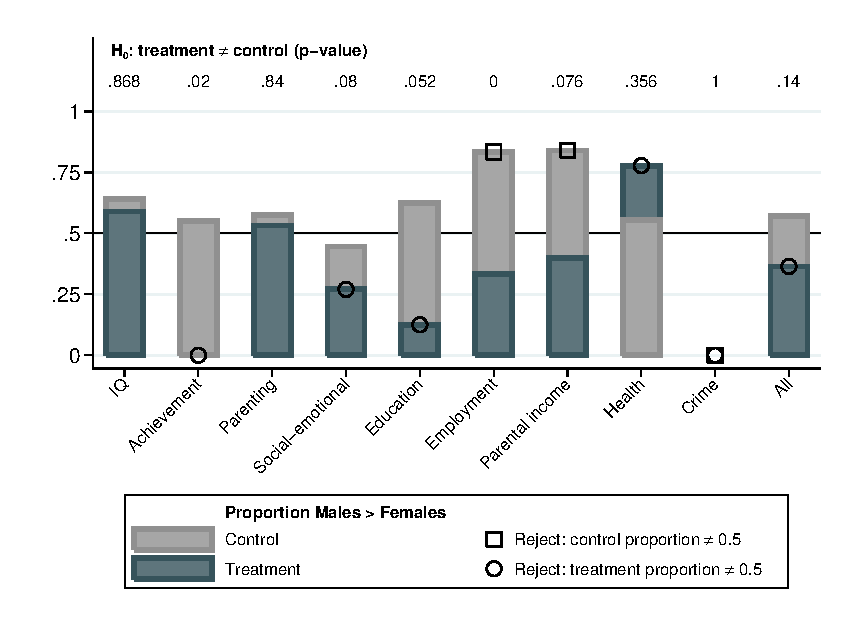
\includegraphics[width=\textwidth]{output/gendergaps-treat-vs-fullcontrol}
\footnotesize \justify
Note: These plots show the proportion of outcomes, by outcome category, for which the male mean is larger than the female mean. The standard errors and the $p$-values are computed using 100 bootstraps. The $p$-values are one-sided and test the null hypothesis that the proportion of outcomes is greater than $\frac{1}{2}$. All the variables are coded such that higher values correspond to socially desirable outcomes. The variables that define each outcome category are listed in Appendix~\ref{appendix:gdiff-outcome-list}.
\end{figure}

Table~\ref{tab:proportion-table} summarizes the gender gaps reported in Figure~\ref{fig:proportion}, as well as those that account for the childcare environment of the control-group children. In the control group, the proportion of outcomes for which males do better than females is higher than 50\% for most of the categories, although not all are statistically significant. Exceptions include social-emotional skills and crime, in which females surpass males. Treatment reverses the gaps for achievement, education, employment, parental income, and over all outcomes. It widens the gap for health, with treatment causing males to achieve better health outcomes. Considering controls who stay at home, females have slightly better health outcomes than males. Finally, the males who attend lower-quality preschools do not outperform females on any of the outcome categories associated with cognition, education, and parenting. These measurements are concentrated early in life, indicating an early-life disadvantage that enriched early childcare programs partially correct.

\begin{table}[H]
\centering
\caption{Summary of Proportion of Outcomes Males $>$ Females}
\label{tab:proportion-table}
\begin{threeparttable}
\begin{tabular}{l | c |c |c| c}
\toprule
& (1) & (2) & (3) & (4) \\
Category & Control Group  &  Control Group &  Control Group &  Treatment \\
	&				&	Stay at Home		& Alternative Preschool &  Group \\
\midrule  
IQ 								& \checkmark 	&  \checkmark* 		& $\times$	& \checkmark \\
Achievement						& \checkmark* 	&  \checkmark* 		&$\times$		& $\times$* \\
Social-emotional					& $\times$	& \checkmark 		&$\times$* 	&$\times$ \\
Parenting							& \checkmark	&  \checkmark* 		&$\times$ 	& $\times$ \\
Parental income					&  \checkmark  &\checkmark* 		& $\times$  	& \checkmark \\
Education							& \checkmark 	&\checkmark 		& $\times$ 	&	$\times$* \\
Employment						&  \checkmark* &  \checkmark* 		& $=$ 		&\checkmark* \\
Crime							&  $\times$* 	&  $=$ 			& $\times$* 	&  $\times$* \\
Risky Behavior						& $\times$	& $\times$*		& \checkmark	& $\times$* \\
Health 							& $=$ 		& $\times$ 		& $\times$ 	&  \checkmark *\\
Mental Health						& \checkmark* & \checkmark* 		&	\checkmark &	\checkmark \\

\midrule
All								&  \checkmark &\checkmark*&  $\times$ & $\times$\\
\bottomrule
\end{tabular}
\begin{tablenotes}
\footnotesize
\item Note: This table summarizes comparison of gender gaps across outcome categories by different groups. A \checkmark indicates that the proportion of outcomes in the corresponding category is larger than $\frac{1}{2}$, meaning that males outperform females. A \checkmark* indicates that the proportion is significantly larger than $\frac{1}{2}$. A $\times$ indicates that the proportion is less than $\frac{1}{2}$. A $\times$* indicates that it is significantly less than $\frac{1}{2}$. A $=$ means that the proportion is $\frac{1}{2}$. Column (1) is the difference between males and females in the full control group.  Column (2) is the difference between males and females in the control group only considering those who stayed at home. Column (3) is the difference between males and females in the control group only considering those who attended alternative preschools. Column (4) is the difference between males and females in the treatment group. The variables for each outcome category are listed in Appendix~\ref{appendix:gdiff-outcome-list}.
\end{tablenotes}
\end{threeparttable}
\end{table}

This paper unfolds in the following way. Section~\ref{sec:data} describes our experimental data and its special features. It documents that a considerable proportion of the control group children attend lower quality preschools compared to treatment children. Section~\ref{sec:parameters} defines the treatment effects we estimate and how we summarize them. Section~\ref{sec:treatment-effects} reports the treatment effects overall and by gender and establishes the existence of sharp gender effects in many categories of outcomes. Section~\ref{sec:gender-differences} discusses differences in the proportions of outcomes favoring men by category. Section~\ref{sec:conclusion} discusses the sources of these differences.


%ee \citet{Beeghly-etal_2017_IMHJ,Dayton_2017_IMHJ,Iruka_2017_IMHJ,Schore_2017_IMHJ} for recent findings on the topic of different development of males and females early in life. 